\Chapter{Tesztelés}

Ebben a fejezetben a már elkészült alkalmazás komponenseit szeretném bemutatni működés közben, valamint egy útmutató jellegű leírást adni az alkalmazás használatáról.\newline

A fejlécen látható az oldal emblémája amire kattintva a kezdő oldalt tudjuk elérni bárhonnan, valamint megtalálható még 3 ikon a bejelentkezéshez, az összes verseny és az összes játékos eléréséhez.\newline

Az alkalmazás kezdőlapján (\ref{fig:homeTest} ábra) a terveknek megfelelően szűrve jelennek meg azok a versenyek amelyek még aktívak vagyis, vannak még olyan mérkőzéseik amik nem kerültek befejezésre és nincsen győztese. A "Continue" gombra kattintva ezeknek a versenyeknek az adatlapját tudjuk elérni, valamint a "+ New Tournament" gombbal új versenyt hozhatunk létre.

\begin{figure}[h]
\centering
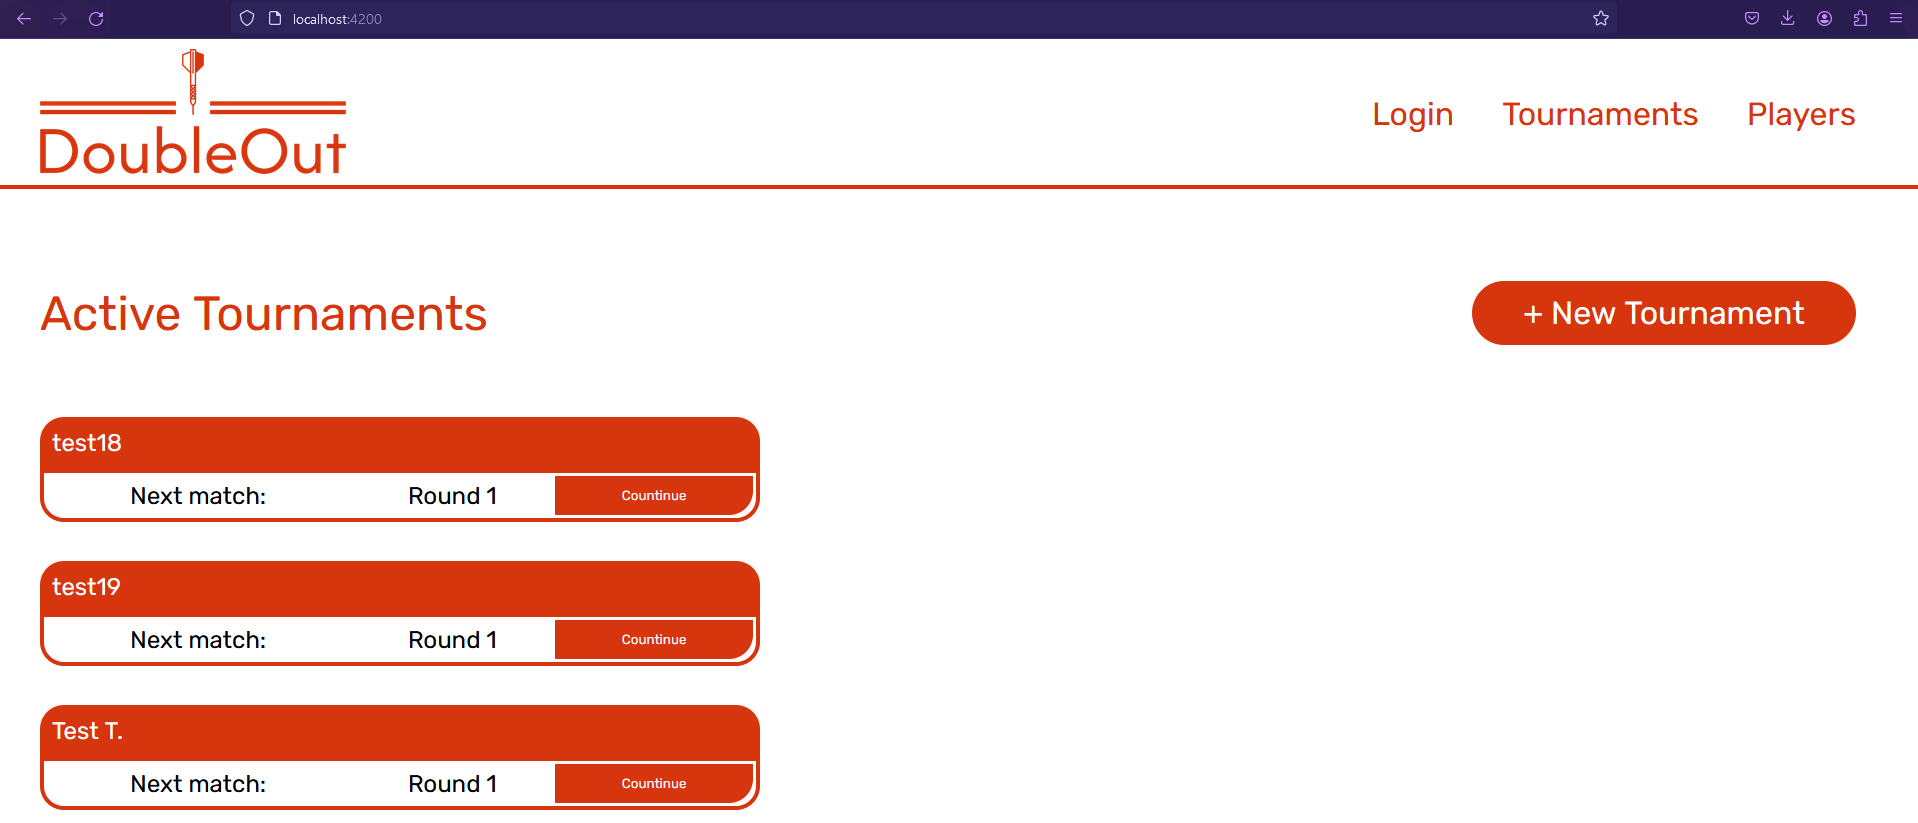
\includegraphics[scale=0.3]{images/HomeTest.png}
\caption{A kezdő oldal futás közben}
\label{fig:homeTest}
\end{figure}

A fejlécen megtalálható "Login" gombra kattintva tudnak a regisztrált felhasználók bejelentkezni (\ref{fig:loginTest} ábra) az e-mail címük és jelszavuk megadásával, azonban az se jelent problémát ha az adott felhasználó még nem regisztrált, hiszen a bejelentkezési oldalról a "Register" gombra kattintva továbbléphetünk a regisztrációs oldalra (\ref{fig:registerTest} ábra), ahol a nevünk, e-mail címünk, jelszavunk megadásával és megerősítésével regisztrálhatnak. Miután bejelentkeztünk vagy regisztráltunk a fejléc "Login" gombja megváltozik a felhasználó nevére amire rákattintva kijelentkezni tudunk.

\begin{figure}[h]
\centering
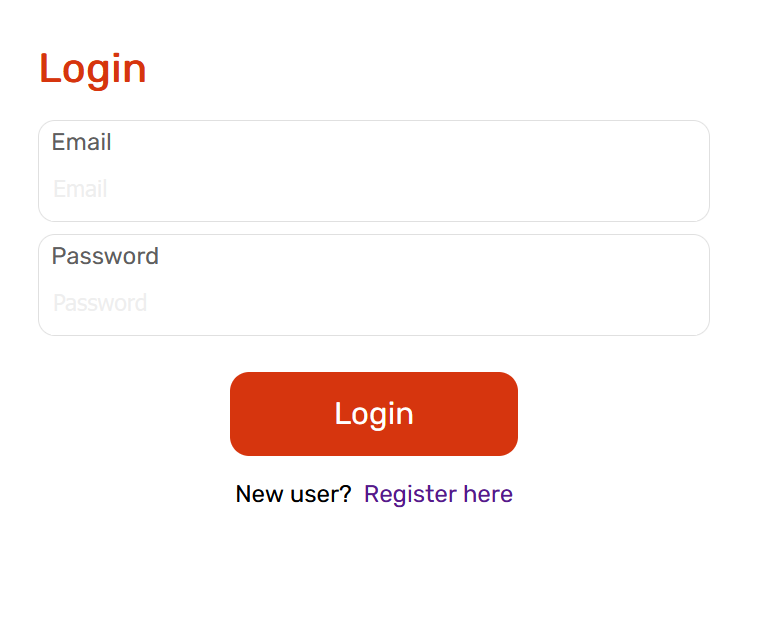
\includegraphics[scale=0.3]{images/LoginTest.png}
\caption{A bejelentkezési oldal futás közben}
\label{fig:loginTest}
\end{figure}

\begin{figure}[h]
\centering
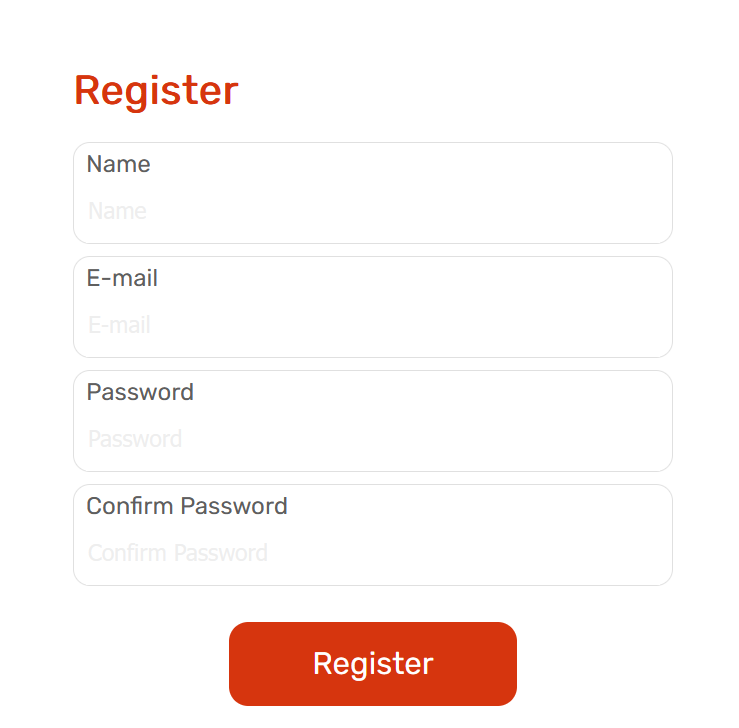
\includegraphics[scale=0.3]{images/RegisterTest.png}
\caption{A regisztrációs oldal futás közben}
\label{fig:registerTest}
\end{figure}

A versenyek oldala (\ref{fig:tournamentsTest} ábra) szinte megegyezik a kezdő oldallal, annyi különbséggel, hogy itt már láthatjuk a befejezett versenyeket is, mint ahogy az az első elemen is látszik.

\begin{figure}[h]
\centering
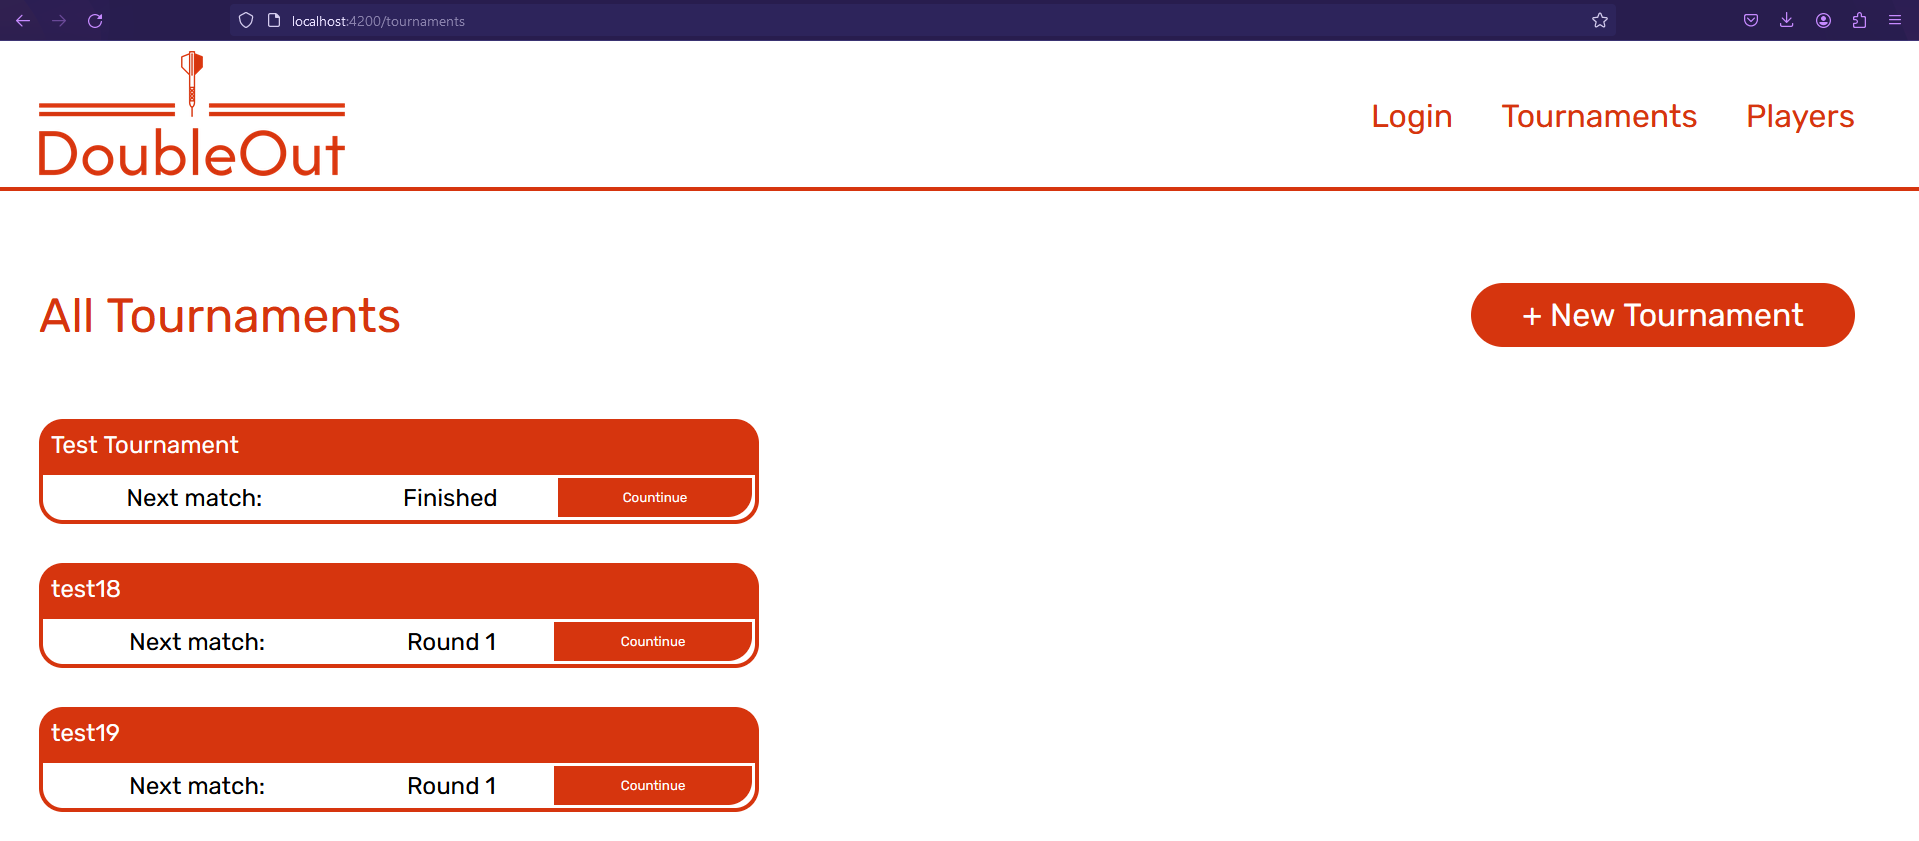
\includegraphics[scale=0.3]{images/TournamentsTest.png}
\caption{A versenyek oldala futás közben}
\label{fig:tournamentsTest}
\end{figure}

Egy verseny létrehozásához (\ref{fig:newTournamentTest} ábra) egy form-ot kell kitöltenünk a verseny nevével, típusával, a játékosok számával, a mérkőzések pontszámával, a győzelemhez szükséges legek számával, valamint azzal az információval, hogy a mérkőzéseken duplával kell-e kiszállni. Ezt követően az "Add Players" gomb megnyomásával hozzáadódnak a játékosok és a megjelenő "Player Name" mezőkben kell kitölteni a résztvevő játékosok neveit. Miután végeztünk az összes lépéssel a "Create Tournament" gombra kattintva létrehozzuk a versenyt.

\begin{figure}[h]
\centering
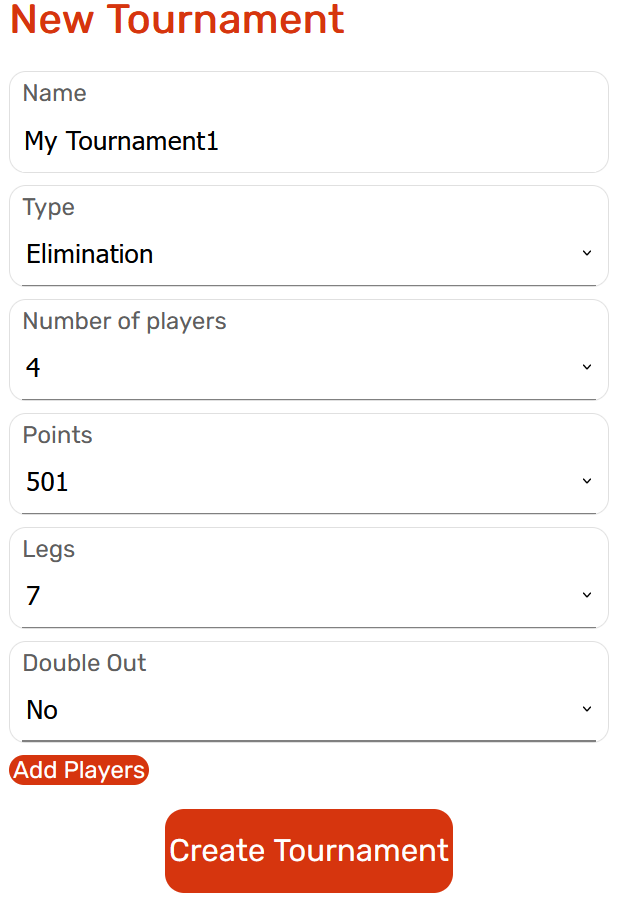
\includegraphics[scale=0.3]{images/NewTournamentTest.png}
\caption{Verseny létrehozása}
\label{fig:newTournamentTest}
\end{figure}

A verseny oldal (\ref{fig:tournamentTest} ábra) bal oldalán láthatóak a hozzátartozó mérkőzések és a view gombra kattintva tudunk továbblépni az adott mérkőzés oldalára, jobb oldalon pedig a verseny statisztikáinak az összesítését láthatjuk, vagyis az összes olyan mérkőzés statisztikájának az összegzését, amelyet a versenyen játszottak le.

\begin{figure}[h]
\centering
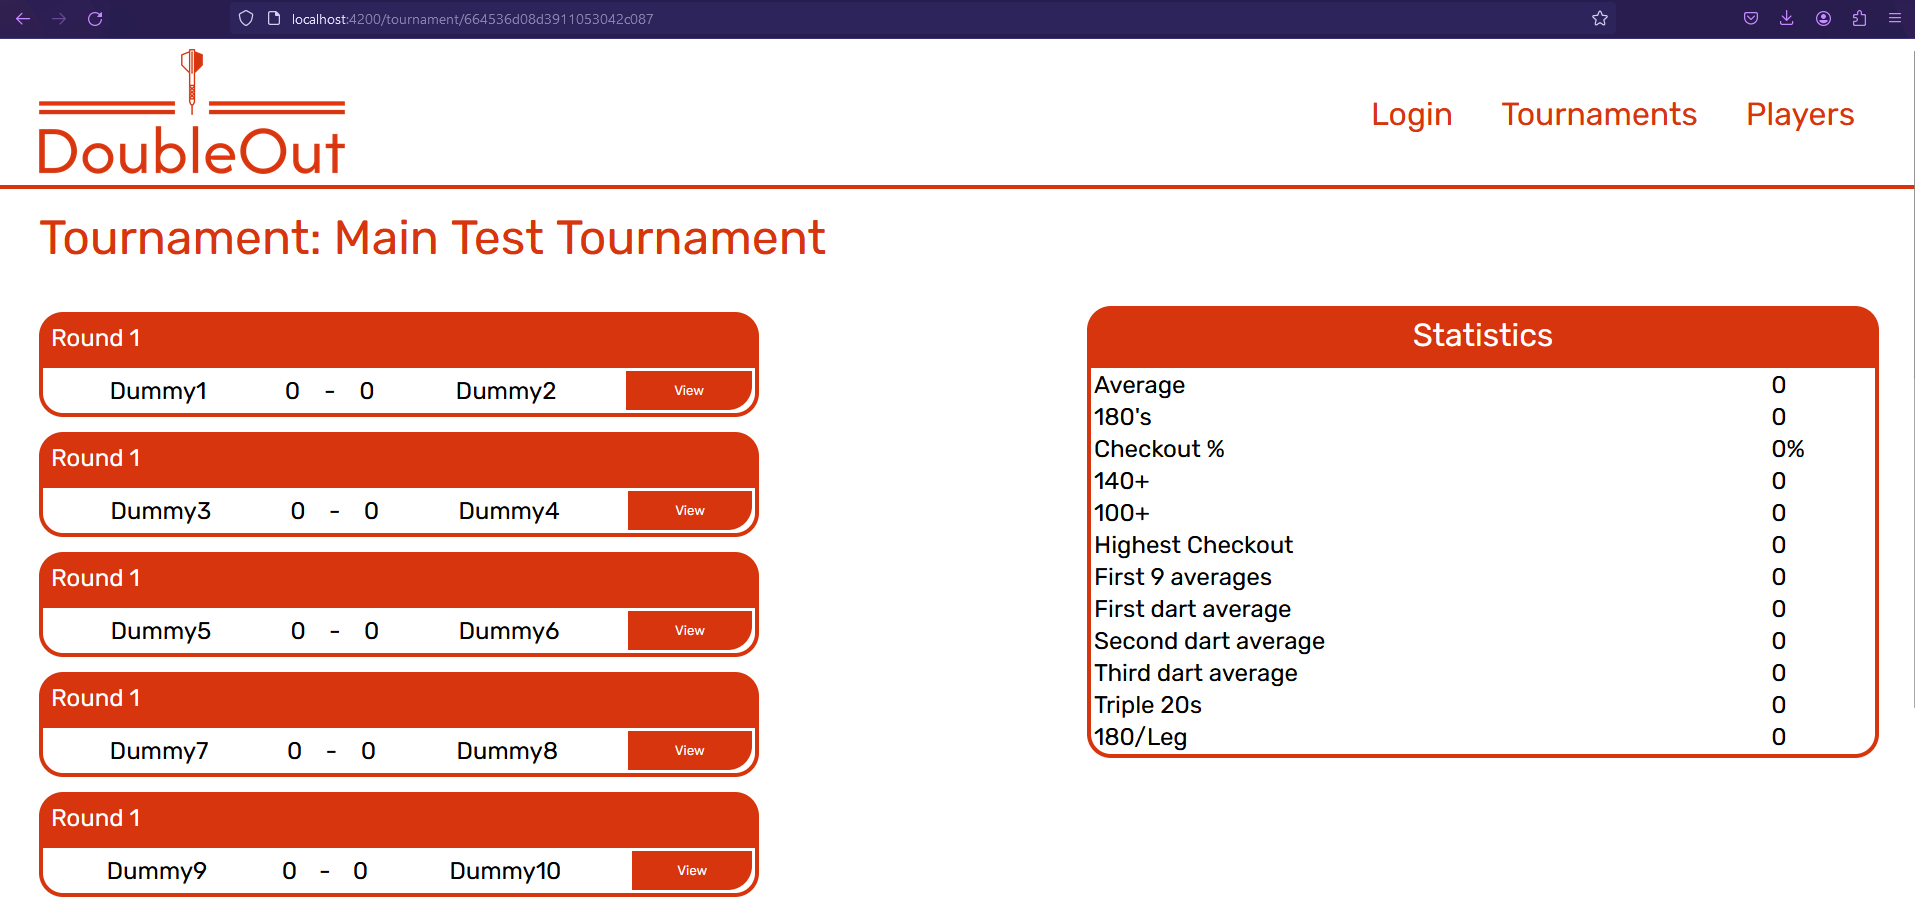
\includegraphics[scale=0.3]{images/TournamentTest.png}
\caption{A verseny oldal futás közben}
\label{fig:tournamentTest}
\end{figure}

A mérkőzés oldalának két fázisa van. Az első fázisban (\ref{fig:matchTest1} ábra) a mérkőzés két játékosát láthatjuk, a mérkőzés statisztikáit, valamint amennyiben a mérkőzést meg nem kezdték el, akkor egy "Start Match" vagy egy "Continue Match" gombot. Erre a gombra kattintva lépünk tovább az oldal második fázisába (\ref{fig:matchTest2} ábra), ami az aktív mérkőzés. Ebben a fázisban az oldal tartalmilag annyiban különbözik, hogy középen megjelenik a pontok rögzítésére használható blokk. Legfelül láthatjuk, hogy melyik játékosnak kell dobni, azaz a beírt értékek ennek a játékosnak a pontjaiból kerülnek majd levonásra, a dobást pedig a "Throw" gomb megnyomásával tudjuk rögzíteni. A dobások után minden alkalommal dinamikusan frissülnek a játékos pontjai, a statisztikák, valamint a dobás értéke kiírásra kerül az adott játékos pontszáma alatt. Amennyiben az egyik játékos megnyerte az aktuális leg-et, akkor frissül az eredmény, a játékosok pontszámai visszaállnak az alaphelyzetbe és a dobott pontszámok is lenullázódnak. Miután valamelyik játékos elérte a győzelemhez szükséges leg-ek számát, akkor megjelenik egy "Finish Match" gomb, amivel befejezhetjük a mérkőzést.

\begin{figure}[h]
\centering
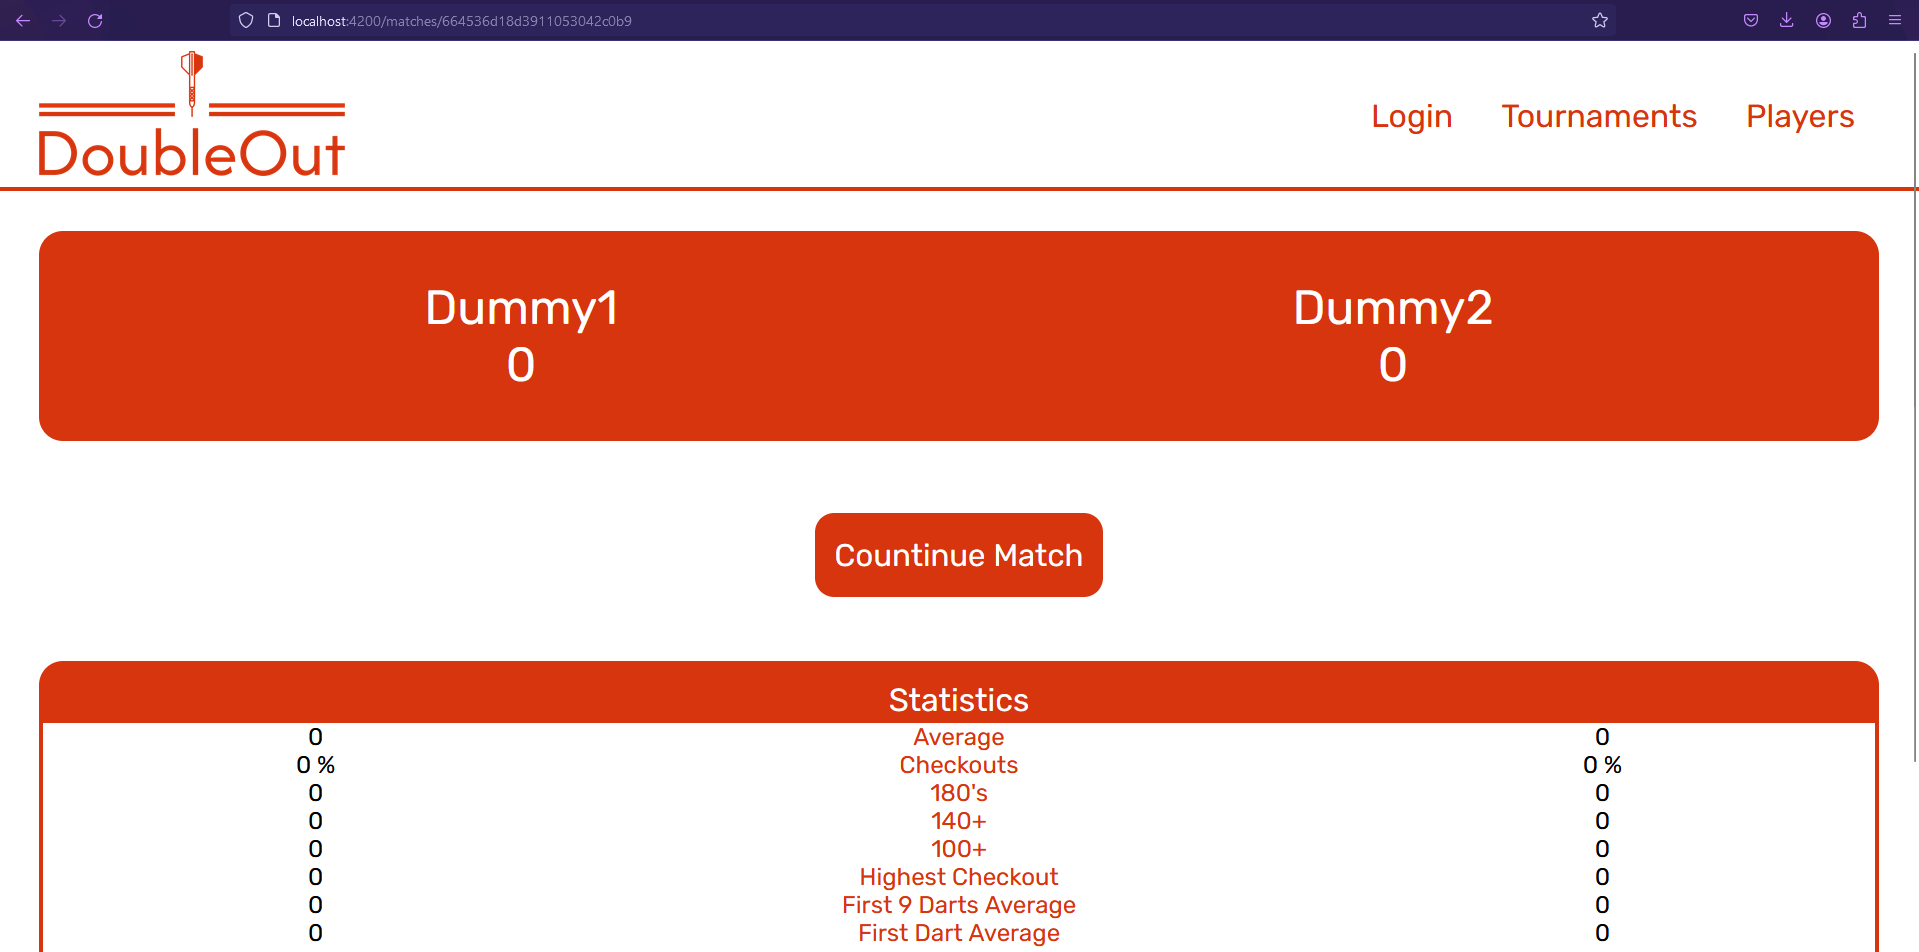
\includegraphics[scale=0.3]{images/MatchTest1.png}
\caption{Egy mérkőzés oldala}
\label{fig:matchTest1}
\end{figure}

\begin{figure}[h]
\centering
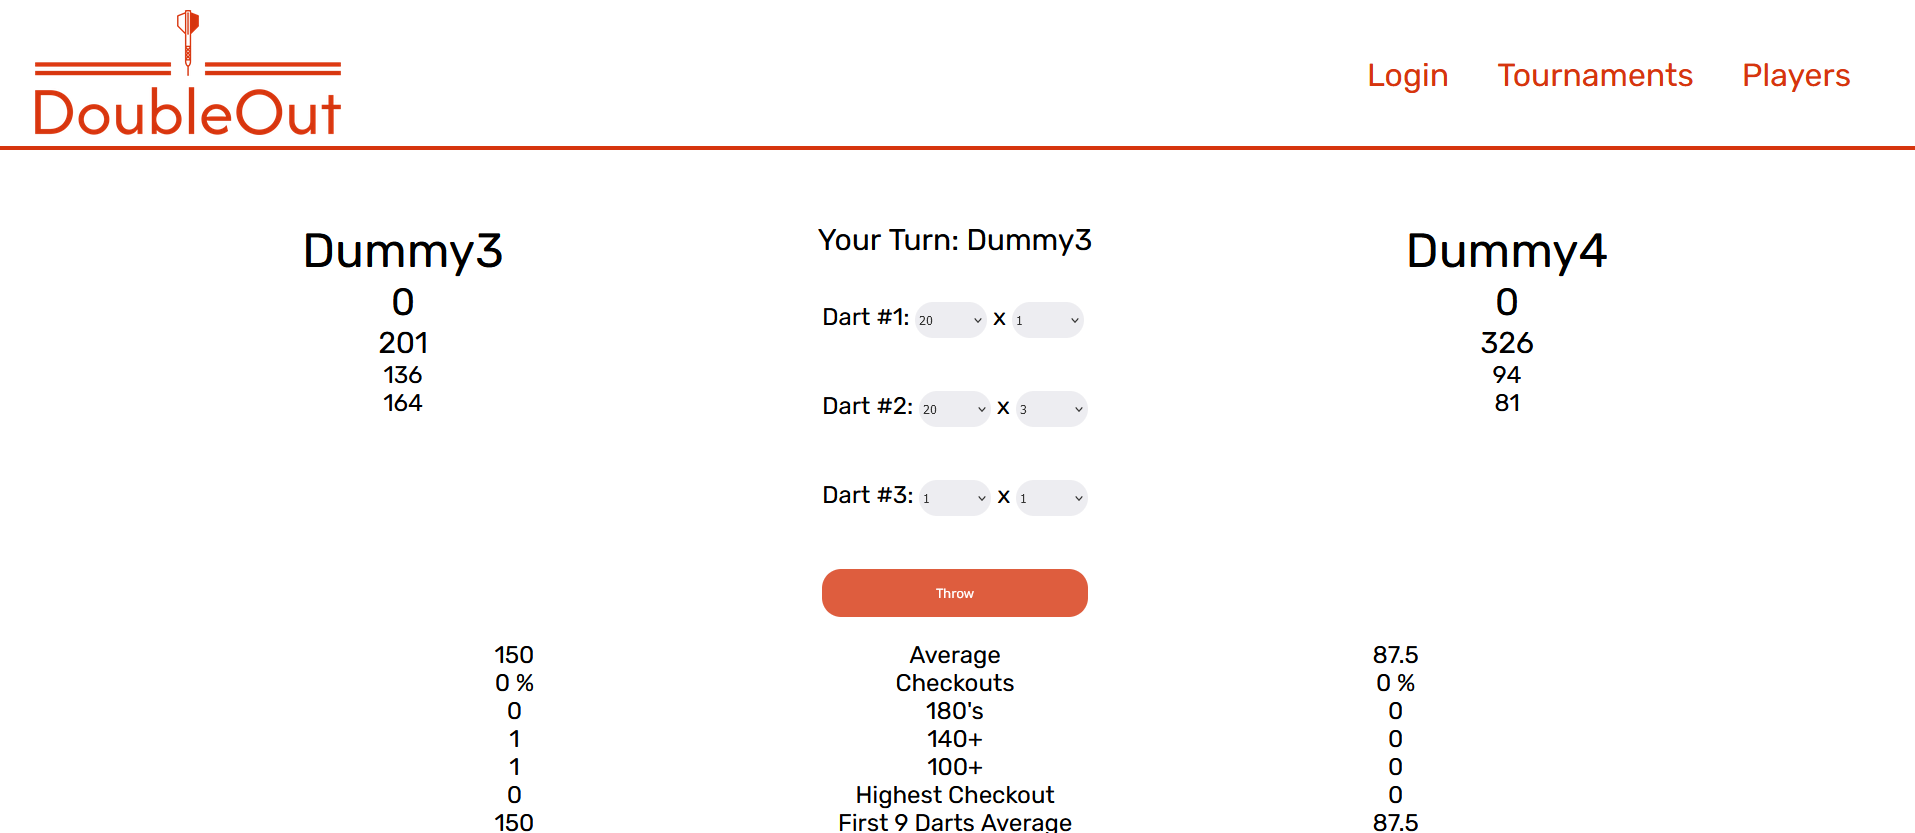
\includegraphics[scale=0.3]{images/MatchTest2.png}
\caption{Egy mérkőzés játék közben}
\label{fig:matchTest2}
\end{figure}

A játékosok oldalán (\ref{fig:playersTest} ábra) kilistázásra kerül minden olyan játékos akik szerepeltek vagy szerepelnek valamelyik versenyen, valamint itt megtalálható egy kereső mező a terveknek megfelelően. Egy játékost kiválasztva tudunk továbblépni az adott játékos adatlapjára. 

\begin{figure}[h]
\centering
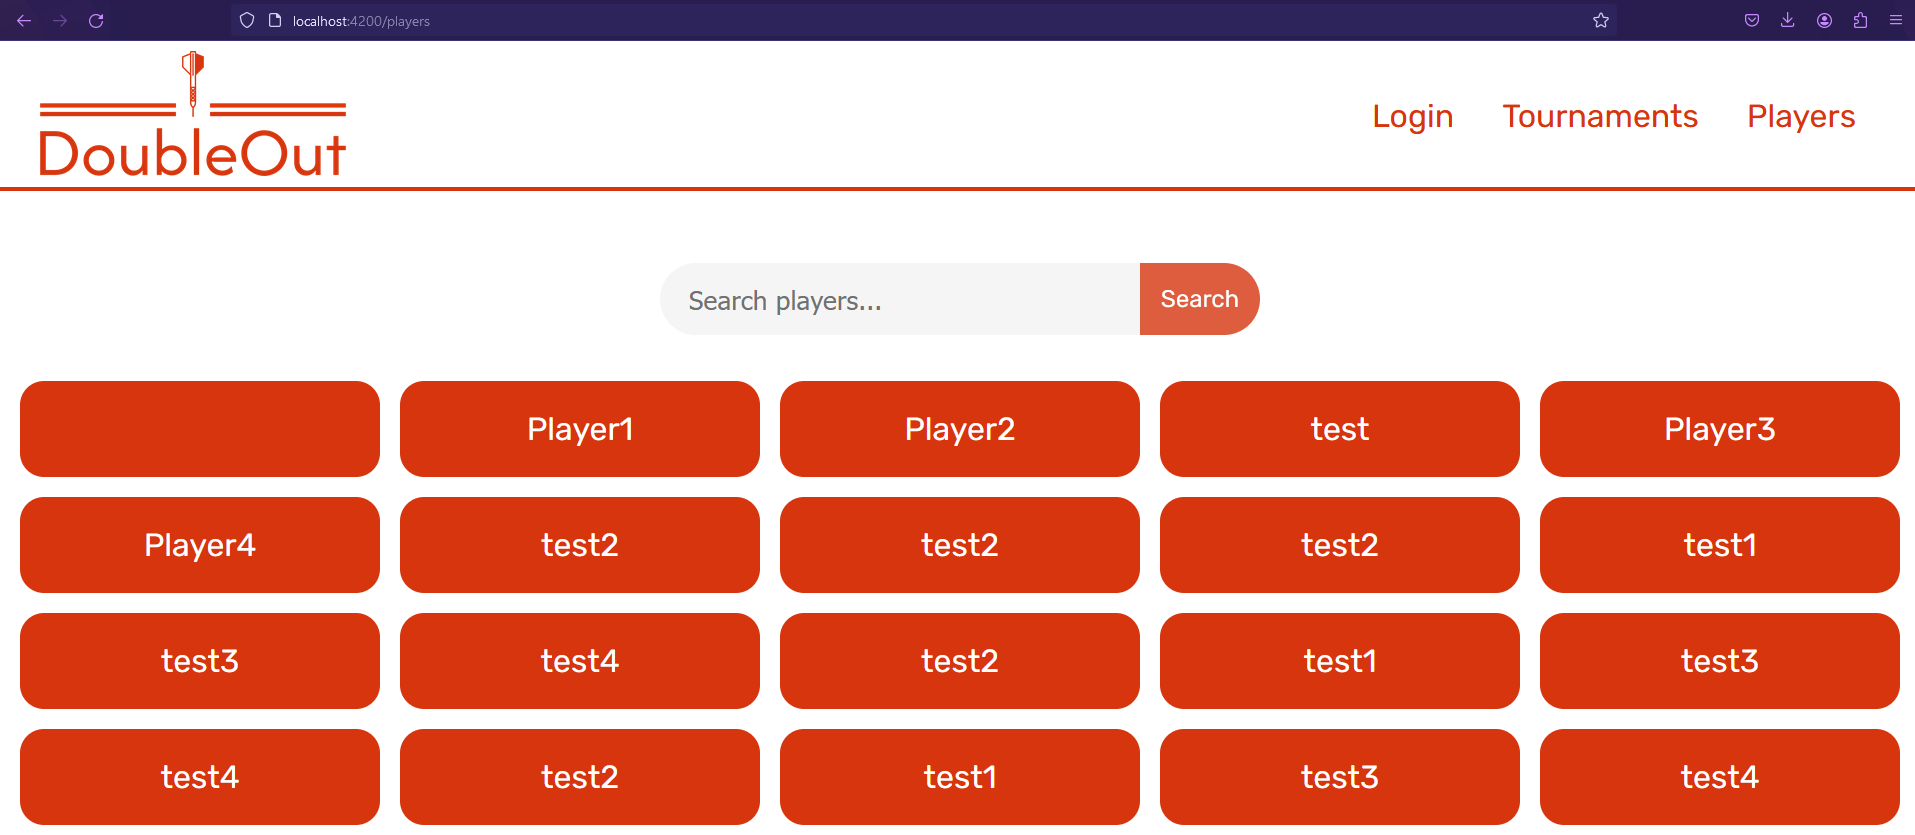
\includegraphics[scale=0.3]{images/PlayersTest.png}
\caption{A játékosok oldala futás közben}
\label{fig:playersTest}
\end{figure}

Egy játékos adatlapján (\ref{fig:playerTest} ábra) megtekinthetőek az adott játékos által lejátszott mérkőzések összesített statisztikái, valamint minden olyan befejezett mérkőzés, amelyben a játékos részt vett. Értelemszerűen a mérkőzés melletti "View" gombra kattintva itt is továbbléphetünk az adott mérkőzés oldalára.

\begin{figure}[h]
\centering
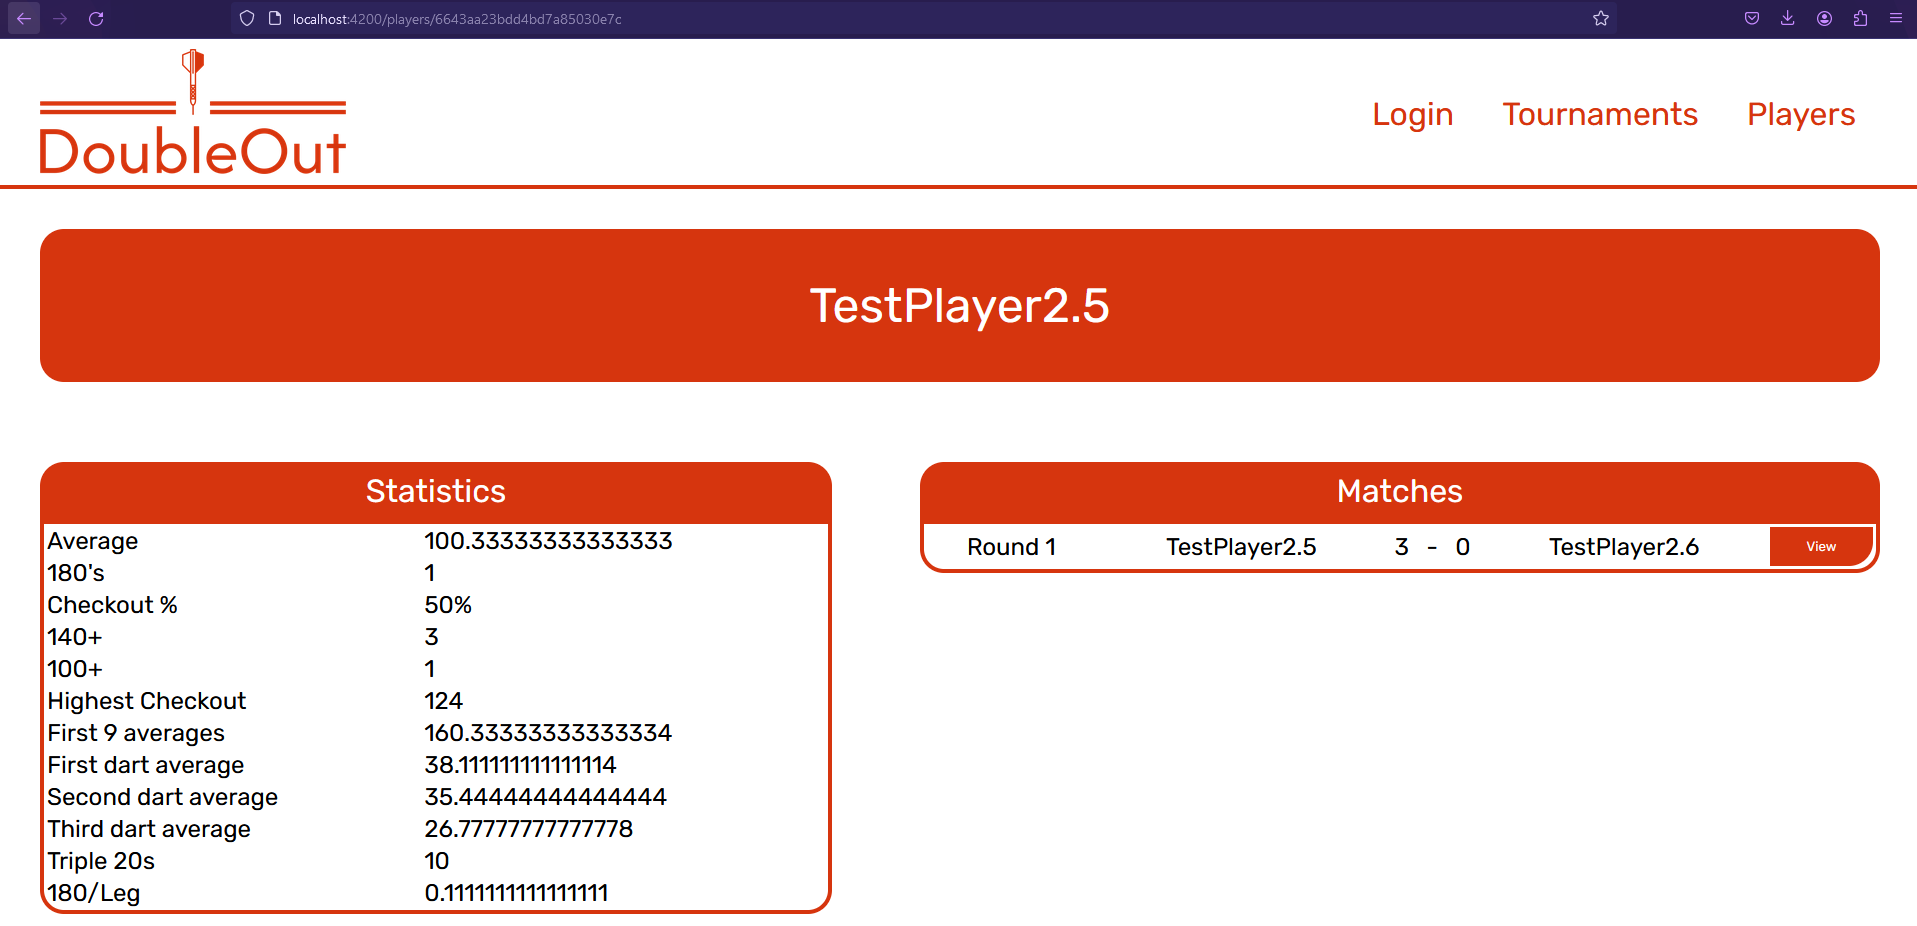
\includegraphics[scale=0.3]{images/PlayerTest.png}
\caption{Egy játékos oldala futás közben}
\label{fig:playerTest}
\end{figure}